%This work is licensed under the Creative Commons
%Attribution-ShareAlike 4.0 International License. To view a copy of
%this license, visit http://creativecommons.org/licenses/by-sa/4.0/ or
%send a letter to Creative Commons, PO Box 1866, Mountain View, CA
%94042, USA.

%This work is licensed under the Creative Commons
%Attribution-ShareAlike 4.0 International License. To view a copy of
%this license, visit http://creativecommons.org/licenses/by-sa/4.0/ or
%send a letter to Creative Commons, PO Box 1866, Mountain View, CA
%94042, USA.

%\documentclass[gray,handout, pdflatex, 11pt]{beamer}
%\documentclass[handout, pdflatex, 11pt]{beamer}

\documentclass[pdflatex, 11pt]{beamer}

\usepackage[utf8]{inputenc}
\usepackage[T1]{fontenc}
\usepackage{calligra}
\usepackage{lmodern}
%\usepackage[italian]{babel}
\usepackage{acronym}
\usepackage{amsmath}
\usepackage{graphicx}
\usepackage{multirow}
\usepackage{listings}
\usepackage{microtype}
\usepackage{bm}
\usepackage{subfig}
\usepackage{acronym}
\usepackage{array}
\usepackage{pifont}
\usepackage{appendixnumberbeamer}
\usepackage{tikz}
\usetikzlibrary{shapes, chains, scopes, shadows, positioning, arrows,
  decorations.pathmorphing, calc, mindmap, petri}

\newcommand{\cmark}{\ding{52}}%{\ding{51}}
\newcommand{\xmark}{\ding{56}}%{\ding{55}}
\newcommand{\hmark}{\ding{42}}%{\ding{43}}
%\newcommand{\cmark}{*}
%\newcommand{\xmark}{x}
%\newcommand{\hmark}{-}

\graphicspath{{img/}}
\lstset{inputpath=../cSrc/}

\definecolor{links}{HTML}{2A1B81}
\hypersetup{colorlinks,linkcolor=links,urlcolor=links}

\definecolor{links}{HTML}{2A1B81}
\hypersetup{colorlinks,linkcolor=,urlcolor=links}


\mode<presentation>{
  \usetheme{Martina}
  %-------------------------1
  %\usetheme{Boadilla}
  %\usecolortheme{beaver}
  %-------------------------1
  %-------------------------2
  %\usetheme{Goettingen}
  %\usecolortheme{sidebartab}
  %-------------------------2
  %\useoutertheme[right]{sidebar}
  %\usefonttheme{default}
  \setbeamercovered{transparent}
  %\setbeameroption{show notes on second screen=right}
  %\setbeamertemplate{navigation symbols}{}
  %\setbeamertemplate{footline}{}

  \bibliographystyle{abbrv}  
  %\renewcommand\bibfont{\scriptsize}
  %\setbeamertemplate{bibliography item}{\textbullet}
  \setbeamertemplate{bibliography item}{\insertbiblabel}
  \setbeamertemplate{itemize item}{\cmark}
  % \setbeamertemplate{itemize subitem}{-}
  \setbeamertemplate{enumerate items}[default]
  \setbeamertemplate{sections/subsections in toc}[square]
}

\newcommand{\backupbegin}{
   \newcounter{finalframe}
   \setcounter{finalframe}{\value{framenumber}}
}
\newcommand{\backupend}{
   \setcounter{framenumber}{\value{finalframe}}
}


%======================================================


\newcommand{\svm}{\textbf{\emph{U-SVM}}}
\newcommand{\svmb}{\textbf{\emph{B-SVM}}}
\newcommand{\lstmng}{\textbf{\emph{B-LSTM}}}
\newcommand{\lstmc}{\textbf{\emph{G-CRNN}}}
\newcommand{\lstmb}{\textbf{\emph{G-LSTM}}}
\newcommand{\maxp}{\textbf{\emph{G-MAX}}}
\newcommand{\softmax}{\textbf{\emph{G-ATT}}}
\newcommand{\maxi}{\textbf{\emph{G-MAXi}}}
\newcommand{\softmaxi}{\textbf{\emph{G-ATTi}}}
\newcommand{\maxh}{\textbf{\emph{G-MAXh}}}
\newcommand{\softmaxh}{\textbf{\emph{G-ATTh}}}
\newcommand{\bert}{\textbf{\emph{BERT}}}
\newcommand{\gru}{\textbf{\emph{G-GRU}}}


\newcommand{\site}{Main-site}
\newcommand{\fullSite}{Full-site}
\newcommand{\type}{Type}
\newcommand{\behaviour}{Behavior}

\newcommand{\matr}[1]{\bm{#1}}
\newcommand{\vect}[1]{\bm{#1}}
\newcommand{\dist}[1]{\mathcal{#1}}

%\newtheorem{definition}{Definition}[section]
%\newtheorem{lemma}[definition]{Lemma}
%\newtheorem{corollary}[definition]{Corollary}
%\newtheorem{theorem}[definition]{Theorem}

\def\RSet{\mathbb{R}}
\def\NSet{\mathbb{N}}
\def\XSet{\mathbb{X}}
\def\YSet{\mathbb{Y}}
\def\HSet{\mathbb{H}}
\def\prob{\mathbb{P}}
\def\expect{\mathbb{E}}
\def\define{\overset{\underset{\mathrm{def}}{}}{=}}

\DeclareMathOperator*{\argmax}{arg\,max}
\DeclareMathOperator*{\argmin}{arg\,min}

\def\loss{\mathcal{L}}

\acrodef{han}[HAN]{Hierarchical Attention Network}
\acrodef{max}[MM]{Max Model}
\acrodef{softmax}[AM]{Attention Model}
\acrodef{maxi}[MMi]{Max Model interpretable}
\acrodef{maxh}[MMh]{Max Model hierarchical}
\acrodef{softmaxh}[AMh]{Attention Model hierarchical}
\acrodef{srm}[SRM]{Structural Risk Minimization}
\acrodef{vcd}[VC-dimension]{Vapnik-Chervonenkis dimension}
\acrodef{pac}[PAC]{Probably Approximately Correct}
\acrodef{iid}[i.i.d.]{indipendently and identically distributed}
\acrodef{ml}[ML]{Machine Learning}
\acrodef{ai}[AI]{Artificial Intelligence}
\acrodef{erm}[ERM]{Empirical Risk Minimization}
\acrodef{rtt}[RTT]{Registro Tumori della Toscana, Tumor Registry of Tuscany}
\acrodef{icdo}[ICD-O]{International Classification of Diseases for Oncology}
\acrodef{icdo1}[ICD-O-1]{International Classification of Diseases for Oncology, first edition}
\acrodef{icdo3}[ICD-O-3]{International Classification of Diseases for Oncology, third edition}
\acrodef{hdr}[HDR]{Hospital Discharge Register}
\acrodef{ehr}[EHR]{Electronic Health Record}
\acrodef{cdf}[CDF]{Cumulative Distribution Function}
\acrodef{an}[AN]{Artificial Neuron}
\acrodef{ann}[ANN]{Artificial Neural Network}
\acrodef{cnn}[CNN]{Convolutional Neural Network}
\acrodef{rnn}[RNN]{Recurrent Neural Network}
\acrodef{mlp}[MLP]{Multilayer Perceptron}
\acrodef{lstm}[LSTM]{Long Short-Term Memory}
\acrodef{sgd}[SGD]{Stochastic Gradient Descend}
\acrodef{glove}[GloVe]{Global Vectors}
\acrodef{nb}[NB]{Naive Bayes}
\acrodef{svm}[SVM]{Support Vector Machine}
\acrodef{tfidf}[TF-IDF]{Term-Frequency Inverse-Document-Frequency}
\acrodef{map}[MAP]{Mean Average Precision}
\acrodef{relu}[ReLU]{Rectified Linear Unit}
\acrodef{gru}[GRU]{Gated Recurrent Unit}
\acrodef{nlp}[NLP]{Natural Language Processing}
\acrodef{bert}[BERT]{Bidirectional Encoder Representations from Transformers}
\acrodef{mlm}[MLM]{Masked Language Model}
\acrodef{nsp}[NSP]{Next Sentence Prediction}

\newcommand\floatwidth{0.9\textwidth}
\newcommand\attTableIcdoWidth{2.5cm}
\newcommand\attTableTextWidth{10cm}
\newlength\lunderset
\newlength\rulethick
\lunderset=1.7pt\relax
\rulethick=.8pt\relax
\def\stackalignment{l}
\newcommand\att[4][1]{\setbox0=\hbox{#2}%
  \stackunder[#1\lunderset-\rulethick]{\strut#2}{\color{#3!#4}\rule{\wd0}{\rulethick}}}

\definecolor{att}{rgb}{0, 1, 0}
\definecolor{attb}{rgb}{1, 0, 0}
\newcommand{\attvisB}[3]{\tikz[overlay]\node[fill=att!#2,inner sep=1pt, anchor=text, rectangle, rounded corners=1mm,draw=attb!#3] {#1};\phantom{#1}}

\makeatletter
  \providecommand*\setfloatlocations[2]{\@namedef{fps@#1}{#2}}
\makeatother
\setfloatlocations{figure}{htbp}
\setfloatlocations{table}{htbp}

\newcommand{\dataLabelScale}{0.6}
\newcommand{\schemeNodeDistance}{0.5cm}

\tikzstyle{every neuron}=[circle, draw, minimum size=1cm]
\tikzstyle{bias}=[circle,draw]
\tikzstyle{operation}=[circle,draw]
\tikzstyle{activation}=[draw]
\tikzstyle{layer}=[draw,minimum size=1cm]
\tikzstyle{delay}=[draw,minimum size=0.5cm,fill=black]
\tikzstyle{neuron missing}=[draw=none, scale=4,text height=0.333cm,execute at begin node=\color{black}$\vdots$]
\tikzstyle{vmissing}=[draw=none, scale=4,text height=0.333cm,execute at begin node=\color{black}$\vdots$]
\tikzstyle{hmissing}=[draw=none, scale=4,text width=0.41cm,execute at
begin node=\color{black}$\cdots$]
\tikzstyle{line}=[]
\tikzstyle{arrow}=[->, >=stealth]
\tikzstyle{arrowInverse}=[<-, >=stealth]
\tikzstyle{vectorLine}=[line width=0.6mm]
\tikzstyle{vectorArrow}=[->, >=stealth, line width=0.6mm]
\tikzstyle{border}=[draw]
\tikzstyle{dataBlock}=[draw,minimum size=1cm, minimum height=2cm, double copy shadow={shadow xshift=-0.5ex, shadow yshift=-0.5ex}, fill=white]
\tikzstyle{layer}=[draw,minimum height=2cm]
\tikzstyle{joined}=[join=by {->}]
\tikzstyle{support}=[coordinate,join=by {-}]
\tikzstyle{dataLabel}=[scale=\dataLabelScale]

\newcommand\nodeInput{} % just for safety
\def\nodeInput(#1){%
  \node[dataBlock,joined,scale=\dataLabelScale] (#1) {$200$};
}

\newcommand\nodeEmbedding{} % just for safety
\def\nodeEmbedding(#1){%
  \node[layer,joined] (#1) {\rotatebox{90}{Embed}};
}

\newcommand\nodeGlove{} % just for safety
\def\nodeGlove(#1){%
  \node[layer,joined] (#1) {\rotatebox{90}{GloVe}};
}

\newcommand\nodeConv{} % just for safety
\def\nodeConv(#1){%
  \node[layer,joined] (#1) {\rotatebox{90}{Conv 2}};
}

\newcommand\nodeLstm{} % just for safety
\def\nodeLstm(#1){%
  \node[layer,joined] (#1) {\rotatebox{90}{Bi. LSTM}};
}

\newcommand\nodeAvg{} % just for safety
\def\nodeAvg(#1){%
  \node[layer,joined] (#1) {\rotatebox{90}{Avg pool}};
}

\newcommand\nodeRelu{} % just for safety
\def\nodeRelu(#1){%
  \node[layer,joined] (#1) {\rotatebox{90}{ReLU}};
}

\newcommand\nodeSoftmax{} % just for safety
\def\nodeSoftmax(#1){%
  \node[layer,joined] (#1) {\rotatebox{90}{Softmax}};
}




% \usebackgroundtemplate
% {
%   \begin{tikzpicture}
%     \node[opacity=0.1] {
\includegraphics[]{img/logoUnifi.png}};
% %    \node[opacity=0.04] {
\includegraphics[scale=1]{img/logoUnifi.eps}};
%   \end{tikzpicture}
% }



\begin{document}

\title[]{\textbf{Classification of cancer pathology reports with Deep
  Learning methods}}
\date[5 November 2019]{5 November 2019}
%\subtitle{Master degree thesis}
\institute[University of Florence]{
  
\includegraphics[width=5cm]{img/logoUnifiName.eps}
}

\author[Stefano Martina]{
  \begin{center}
    \begin{tabular}{lr}
      Stefano \textsc{Martina}\\
      \href{mailto:stefano.martina@unifi.it}{stefano.martina@unifi.it}\\
    \end{tabular}
  \end{center}
}


% \titlegraphic{
%   \vspace{-0.5cm}
%   \tiny
%   \href{http://creativecommons.org/licenses/by-sa/4.0/}{
\includegraphics[width=1cm]{img/logoCC.png}}
%   This work is licensed under a
%   \href{http://creativecommons.org/licenses/by-sa/4.0/}{Creative
%     Commons Attribution-ShareAlike 4.0 International License}.
% }


\begin{frame}[plain]
  \titlepage
\end{frame}

\begin{frame}{Overview}
  \tableofcontents
\end{frame}

\section{Introduction}

\subsection{Cancer registries}

\begin{frame}{Cancer}
  
\end{frame}

\begin{frame}{Cancer registries}
  \begin{itemize}
  \item \alert{Collect} administrative and clinical data of a specific region
  \item \alert{Identify} new cancer diagnoses
  \item Provide \alert{details} on diagnoses and outcomes 
  \item \alert{Manual} classification of reports
  \end{itemize}
\end{frame}

\subsection{\acs{icdo}}

\begin{frame}{\acs{icdo3}}
  \begin{itemize}
  \item International \alert{classification} standard
  \item Specialization to \alert{oncology} domain
  \end{itemize}
  \begin{block}{\acf{icdo3}}
      \begin{itemize}
      \item Topography: \texttt{Cmm.s} where \texttt{mm} is the
        \alert{main} site and \texttt{s} the \alert{subsite}
      \item Morphology: \texttt{tttt/b} where \texttt{tttt} is the
        cell \alert{type} and \texttt{b} the \alert{behavior}
      \end{itemize}
  \end{block}
\end{frame}

\subsection{Scientific questions}

\begin{frame}{Scientific questions}
  \begin{description}
  \item[Q1] Implement \alert{large scale} study on deep learning
    applied to pathology reports, existing works are on
    \begin{itemize}
    \item \alert{small} datasets or
    \item \alert{few} classes
    \end{itemize}
  \item[Q2] Apply \alert{novel} deep learning techniques, like
    \alert{attention} models and \alert{acs{bert}}
  \item[Q3] \alert{Compare} classical \alert{bag-of-words} techniques with
    newer deep learning techniques in this domain
  \item[Q4] \alert{Compare} novel \alert{attention}-based and
    \alert{hierarchical} techniques with simpler models
  \item[Q5] \alert{Investigate} the contribution and applicability of
    \alert{unsupervised} learning techniques on uncommon text corpora
  \item[Q6] \alert{Investigate} the possibility to give
    \alert{interpretation} to deep learning models
  \end{description}
\end{frame}


\section{Machine Learning}

\begin{frame}{\acf{nlp}}
  
\end{frame}

\begin{frame}{\acf{tfidf}}
  
\end{frame}

\begin{frame}{\acf{svm}}
  
\end{frame}

\subsection{\acs{rnn}}

\begin{frame}{\acf{rnn}}
  \begin{figure}
    \centering
    % \subfigure[]{
    \subfloat[\label{fig:rnn1}]{
      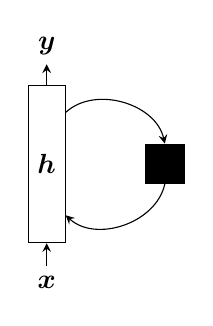
\begin{tikzpicture}[x=1.5cm, y=1.5cm]
        \node [] (input) at (0,0) {$\vect{x}$};
        
        \node [layer] (state) at (0,1) {$\vect{h}$};
        \node [delay] (delay) at (1,1) {};
        
        \node [] (output) at (0,2) {$\vect{y}$};
        
        \draw [arrow] (input) -- (state);
        \draw [arrow] (state) -- (output);
        \draw (state) edge[arrow, bend left=60] (delay.north);
        \draw (delay.south) edge[arrow, bend left=60] (state);
      \end{tikzpicture}
    }\hfill
    % \subfigure[]{
    \subfloat[\label{fig:rnn2}]{
      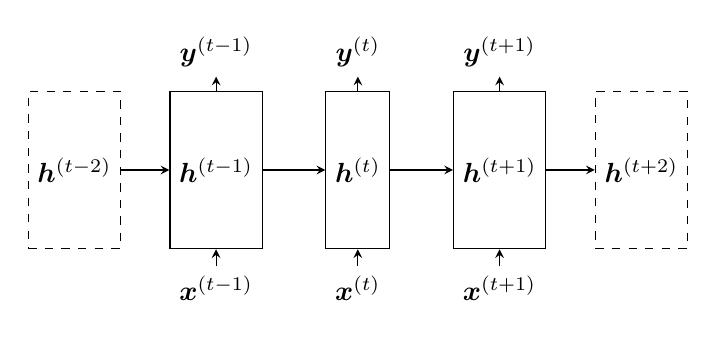
\begin{tikzpicture}[x=1.5cm, y=1.5cm]
        \foreach \l [count=\i] in {t-1,t,t+1}{
          \node [] (input-\i) at (\i*1.2,0) {$\vect{x}^{(\l)}$};
          \node [layer] (state-\i) at (\i*1.2,1) {$\vect{h}^{(\l)}$};
          \node [] (output-\i) at (\i*1.2,2) {$\vect{y}^{(\l)}$};
          
          \draw [arrow] (input-\i) -- (state-\i);
          \draw [arrow] (state-\i) -- (output-\i);
        }
        \node [layer, dashed] (state-l) at (0,1) {$\vect{h}^{(t-2)}$};
        \node [layer, dashed] (state-r) at (4*1.2,1) {$\vect{h}^{(t+2)}$};
        
        \draw [arrow] (state-l) -- (state-1);
        \draw [arrow] (state-1) -- (state-2);
        \draw [arrow] (state-2) -- (state-3);
        \draw [arrow] (state-3) -- (state-r);
      \end{tikzpicture}
    }
    \caption{\acs{rnn}, folded (a) and unfolded (b) models.}
    %\label{fig:rnn}
  \end{figure}
  \begin{equation*}
    \vect{h}^{(t)} = f(\vect{h}^{(t-1)}, \vect{x}^{(t)}; \vect{\theta})
  \end{equation*}
\end{frame}

\begin{frame}{\acf{lstm}}
  \vspace{-0.85cm}
  \begin{figure}
  \centering
  % \subfigure[]{
  \subfloat[]{
    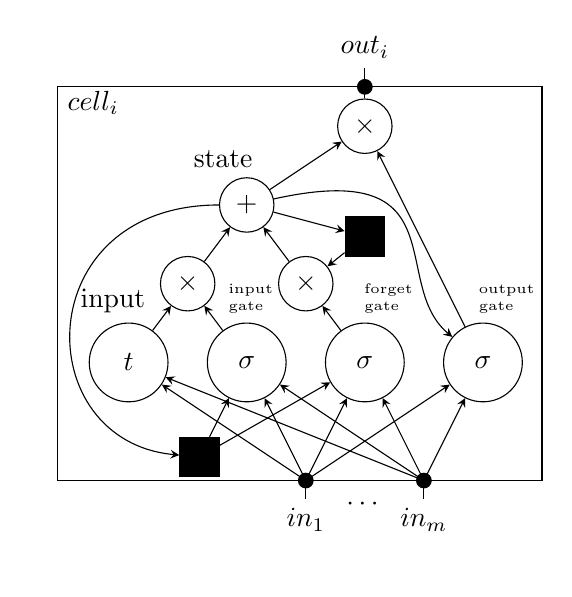
\begin{tikzpicture}[x=1.5cm, y=1cm]
      \node at (1,-0.5) {};

      \node[delay] (delay1) at (1.6,0.8) {};
      \coordinate (input1) at (2.5,0.5);
      \coordinate (input2) at (3.5,0.5);
      \node[] (input01) at (2.5,0) {$in_1$};
      \node[] (input02) at (3.5,0) {$in_m$};
      \node[] at (3,0.2) {$\cdots$};
      \node[every neuron, label={[xshift=-2mm]input}] (inputN) at (1,2) {$t$};
      \node[every neuron, label={[xshift=0.5mm, align=left, font=\tiny] input\\gate}] (inputGate) at (2,2) {$\sigma$};
      \node[every neuron, label={[xshift=3mm, align=left, font=\tiny] forget\\gate}] (forgetGate) at (3,2) {$\sigma$};
      \node[every neuron, label={[xshift=3mm, align=left, font=\tiny] output\\gate}] (outputGate) at (4,2) {$\sigma$};
      \node[operation] (inputTimes) at (1.5, 3) {$\times$};
      \node[operation, label={[xshift=-3mm]state}] (state) at (2, 4) {$+$};
      \node[delay] (delay2) at (3.0,3.6) {};
      \node[operation] (forgetTimes) at (2.5, 3) {$\times$};
      \node[operation] (outputTimes) at (3, 5) {$\times$};
      \coordinate (output1) at (3,5.5);
      \node (output2) at (3,6) {$out_i$};
      \node at (0.7,5.3) {$cell_i$};

      \fill[black] (input1) circle (1mm);
      \fill[black] (input2) circle (1mm);
      \fill[black] (output1) circle (1mm);
      
      \foreach \n in {input1, input2}{
        \foreach \m in {inputN, inputGate, forgetGate, outputGate}{
          \draw[arrow] (\n) -- (\m);
        }
      }
      \foreach \m in {inputGate, forgetGate}{
        \draw[arrow] (delay1) -- (\m);
      }

      \draw[arrow] (inputN) -- (inputTimes);
      \draw[arrow] (inputGate) -- (inputTimes);
      \draw[arrow] (forgetGate) -- (forgetTimes);
      \draw[arrow] (inputTimes) -- (state);
      \draw[arrow] (forgetTimes) -- (state);
      \draw [arrow] (state) ..  controls  (0.15,4) and (0.15,1) ..  (delay1);
      \draw [arrow] (state) ..  controls  (3.8,4.6) and (3.2,3) ..  (outputGate);
      \draw[arrow] (state) -- (delay2);
      \draw[arrow] (delay2) -- (forgetTimes);
      \draw[arrow] (state) -- (outputTimes);
      \draw[arrow] (outputGate) -- (outputTimes);
      \draw[line] (outputTimes) -- (output1);
      \draw[line] (output1) -- (output2);
      \draw[line] (input01) -- (input1);
      \draw[line] (input02) -- (input2);

      \path[border] (0.4,0.5) -- (4.5,0.5) -- (4.5,5.5) -- (0.4,5.5) -- (0.4,0.5); 
      

    \end{tikzpicture}
    \label{fig:lstm1}
  }\hfill
  % \subfigure[]{
  \subfloat[]{
    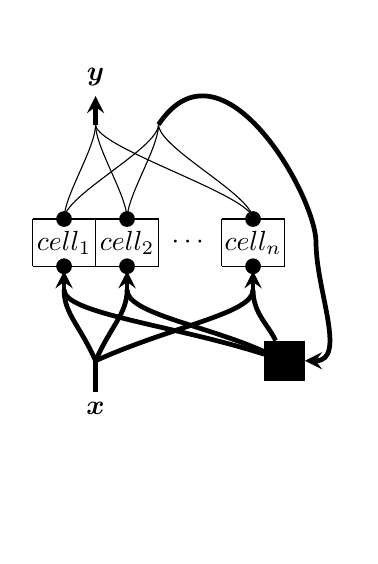
\begin{tikzpicture}[x=0.8cm, y=0.6cm]
      \node at (1,-2.5) {};

      % \draw[step=1.0,black,thin] (0,3) grid (4,4);
      \draw[step=1.0,black,thin] (0,3) grid (2,4);
      \draw[step=1.0,black,thin] (3,3) grid (4,4);
      \coordinate (input1) at (0.5,3);
      \coordinate (input2) at (1.5,3);
      \coordinate (input3) at (3.5,3);
      \coordinate (inputM1) at (0.5,2.5);
      \coordinate (inputM2) at (1.5,2.5);
      \coordinate (inputM3) at (3.5,2.5);
      \coordinate (output1) at (0.5,4);
      \coordinate (output2) at (1.5,4);
      \coordinate (output3) at (3.5,4);

      \coordinate (outputM) at (2,6);
      \coordinate (outputTM) at (1,6);
      
      \node at (0.5, 3.5) {$cell_1$};
      \node at (1.5, 3.5) {$cell_2$};
      \node at (2.5, 3.5) {$\cdots$};
      \node at (3.5, 3.5) {$cell_n$};
      \coordinate (pass) at (4.5, 3.5);
      \node (inputT) at (1,0) {$\vect{x}$};
      \coordinate (inputTM) at (1,1);
      \node (outputT) at (1,7) {$\vect{y}$};

      \node[delay] (delay) at (4,1) {};

      \foreach \c in {input1, input2, input3, output1, output2, output3}{
        \fill[black] (\c) circle (1mm);
      }

      \foreach \c in {inputM1, inputM2, inputM3}{
        \draw [vectorLine] (delay) ..  controls
        ($0.5*(delay)+0.5*(\c)$) and ($(\c)-(0,0.5)$) ..  (\c);
        \draw [vectorLine] (inputTM) ..  controls
        ($0.5*(inputTM)+0.5*(\c)$) and ($(\c)-(0,0.5)$) ..  (\c);
      }

      \foreach \c in {1, 2, 3}{
        \draw[vectorArrow] (inputM\c) -- ($(input\c)-(0,0.1)$);
      }

      \foreach \c in {output1, output2, output3}{
        \draw [line] (\c) ..  controls  ($(\c)+(0,0.5)$) and
        ($(outputM)-(0,0.5)$) ..  (outputM);
        \draw [line] (\c) ..  controls  ($(\c)+(0,0.5)$) and
        ($(outputTM)-(0,0.5)$) ..  (outputTM);
      }

      %\draw [vectorArrow] (outputM) ..  controls  ($(outputM)+(1,2)$) and ($(delay)+(1,0)$) ..  (delay);
      \draw [vectorArrow]
      (outputM) ..
      controls  ($(outputM)+(1,2)$) and ($(pass)+(0,1)$) ..
      (pass) ..
      controls  ($(pass)-(0,1)$) and ($(delay)+(1,0)$) ..
      (delay);
      \draw[vectorLine] (inputT) -- (inputTM);
      \draw[vectorArrow] (outputTM) -- (outputT);
    \end{tikzpicture}
    \label{fig:lstm2}
  }
  \caption{memory cell (a), and general
    scheme (b). The black box is a delay}
  %\label{fig:lstm}
\end{figure}
\end{frame}

\begin{frame}{\acf{gru}}
  \vspace{-0.8cm}
\begin{figure}
  \centering
  % \subfigure[]{
  \subfloat[]{
    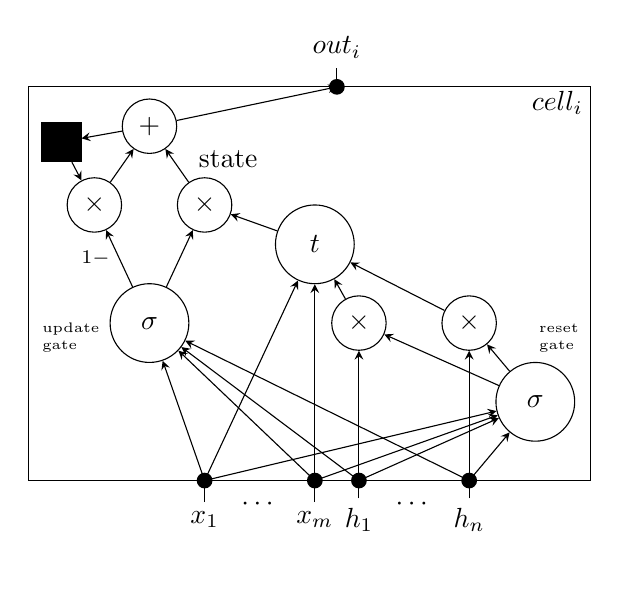
\begin{tikzpicture}[x=1.4cm, y=1cm]
      \node at (1,-0.5) {};

      \coordinate (input1) at (1,0.5);
      \coordinate (input2) at (2,0.5);
      \coordinate (input3) at (2.4,0.5);
      \coordinate (input4) at (3.4,0.5);
      \node[] (input01) at (1,0) {$x_1$};
      \node[] (input02) at (2,0) {$x_m$};
      \node[] (input03) at (2.4,0) {$h_1$};
      \node[] (input04) at (3.4,0) {$h_n$};
      \node[] at (1.5,0.2) {$\cdots$};
      \node[] at (2.9,0.2) {$\cdots$};
      \node[every neuron, label={[xshift=-10mm, yshift=-10mm, align=left, font=\tiny]update\\gate}] (updateGate) at (0.5,2.5) {$\sigma$};
      \node[every neuron, label={[xshift=3mm, align=left, font=\tiny] reset\\gate}] (resetGate) at (4,1.5) {$\sigma$};
      \node[operation] (updateTimesLeft) at (0, 4) {$\times$};
      \node[operation] (updateTimesRight) at (1, 4) {$\times$};
      \node[operation, label={[xshift=10mm,yshift=-10mm]state}] (state) at (0.5, 5) {$+$};
      \node[delay] (delay) at (-0.3,4.8) {};
      \node[operation] (resetTimesLeft) at (2.4, 2.5) {$\times$};
      \node[operation] (resetTimesRight) at (3.4, 2.5) {$\times$};
      \node[every neuron] (candidateState) at (2,3.5) {$t$};
      \coordinate (output1) at (2.2,5.5);
      \node (output2) at (2.2,6) {$out_i$};
      \node at (4.2,5.3) {$cell_i$};

      \fill[black] (input1) circle (1mm);
      \fill[black] (input2) circle (1mm);
      \fill[black] (input3) circle (1mm);
      \fill[black] (input4) circle (1mm);
      \fill[black] (output1) circle (1mm);
      
      \foreach \n in {input1, input2, input3, input4}{
        \foreach \m in {updateGate, resetGate}{
          \draw[arrow] (\n) -- (\m);
        }
      }

      \foreach \n in {input1, input2, resetTimesLeft, resetTimesRight}{
        \draw[arrow] (\n) -- (candidateState);
      }
      
      \draw[arrow] (updateGate) -- (updateTimesLeft) node[draw=none,fill=none,font=\scriptsize,midway,left] {$1-$};
      \draw[arrow] (updateGate) -- (updateTimesRight);
      \draw[arrow] (updateTimesLeft) -- (state);
      \draw[arrow] (updateTimesRight) -- (state);
      %\draw [arrow] (state) ..  controls  (3.8,4.2) and (3.2,3) ..  (resetGate);
      \draw[arrow] (state) -- (delay);
      \draw[arrow] (delay) -- (updateTimesLeft);
      \draw[arrow] (state) -- (output1);
      \draw[arrow] (input3) -- (resetTimesLeft);
      \draw[arrow] (input4) -- (resetTimesRight);
      \draw[arrow] (resetGate) -- (resetTimesLeft);
      \draw[arrow] (resetGate) -- (resetTimesRight);
      \draw[arrow] (candidateState) -- (updateTimesRight);
      \draw[line] (output1) -- (output2);
      \draw[line] (input01) -- (input1);
      \draw[line] (input02) -- (input2);
      \draw[line] (input03) -- (input3);
      \draw[line] (input04) -- (input4);

      \path[border] (-0.6,0.5) -- (4.5,0.5) -- (4.5,5.5) -- (-0.6,5.5) -- (-0.6,0.5); 
    \end{tikzpicture}
    %\label{fig:gru1}
  }\hfill
  % \subfigure[]{
  \subfloat[]{
    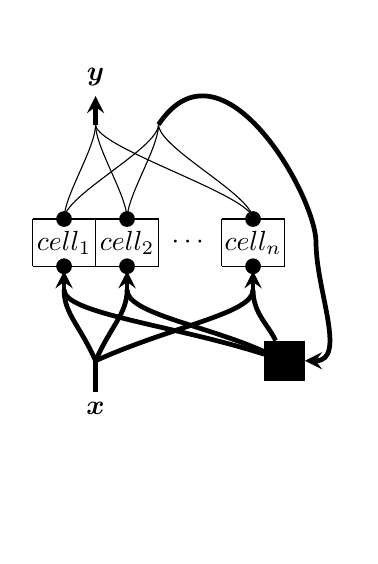
\begin{tikzpicture}[x=0.8cm, y=0.6cm]
      \node at (1,-2.5) {};

      % \draw[step=1.0,black,thin] (0,3) grid (4,4);
      \draw[step=1.0,black,thin] (0,3) grid (2,4);
      \draw[step=1.0,black,thin] (3,3) grid (4,4);
      \coordinate (input1) at (0.5,3);
      \coordinate (input2) at (1.5,3);
      \coordinate (input3) at (3.5,3);
      \coordinate (inputM1) at (0.5,2.5);
      \coordinate (inputM2) at (1.5,2.5);
      \coordinate (inputM3) at (3.5,2.5);
      \coordinate (output1) at (0.5,4);
      \coordinate (output2) at (1.5,4);
      \coordinate (output3) at (3.5,4);

      \coordinate (outputM) at (2,6);
      \coordinate (outputTM) at (1,6);
      
      \node at (0.5, 3.5) {$cell_1$};
      \node at (1.5, 3.5) {$cell_2$};
      \node at (2.5, 3.5) {$\cdots$};
      \node at (3.5, 3.5) {$cell_n$};
      \coordinate (pass) at (4.5, 3.5);
      \node (inputT) at (1,0) {$\vect{x}$};
      \coordinate (inputTM) at (1,1);
      \node (outputT) at (1,7) {$\vect{y}$};

      \node[delay] (delay) at (4,1) {};

      \foreach \c in {input1, input2, input3, output1, output2, output3}{
        \fill[black] (\c) circle (1mm);
      }

      \foreach \c in {inputM1, inputM2, inputM3}{
        \draw [vectorLine] (delay) ..  controls
        ($0.5*(delay)+0.5*(\c)$) and ($(\c)-(0,0.5)$) ..  (\c);
        \draw [vectorLine] (inputTM) ..  controls
        ($0.5*(inputTM)+0.5*(\c)$) and ($(\c)-(0,0.5)$) ..  (\c);
      }

      \foreach \c in {1, 2, 3}{
        \draw[vectorArrow] (inputM\c) -- ($(input\c)-(0,0.1)$);
      }

      \foreach \c in {output1, output2, output3}{
        \draw [line] (\c) ..  controls  ($(\c)+(0,0.5)$) and
        ($(outputM)-(0,0.5)$) ..  (outputM);
        \draw [line] (\c) ..  controls  ($(\c)+(0,0.5)$) and
        ($(outputTM)-(0,0.5)$) ..  (outputTM);
      }

      %\draw [vectorArrow] (outputM) ..  controls  ($(outputM)+(1,2)$) and ($(delay)+(1,0)$) ..  (delay);
      \draw [vectorArrow]
      (outputM) ..
      controls  ($(outputM)+(1,2)$) and ($(pass)+(0,1)$) ..
      (pass) ..
      controls  ($(pass)-(0,1)$) and ($(delay)+(1,0)$) ..
      (delay);
      \draw[vectorLine] (inputT) -- (inputTM);
      \draw[vectorArrow] (outputTM) -- (outputT);
    \end{tikzpicture}
    %\label{fig:gru2}
  }
  \caption{memory cell (a), and general
    scheme (b). The black box is a delay}
  %\label{fig:gru}
\end{figure}
\end{frame}

\begin{frame}{Word vectors}
  \begin{itemize}
  \item \alert{Transforms} words in vectors
  \item \alert{Unsupervised} learning method
  \item \alert{Semantic} relations encoded in vector space geometric relations 
  \end{itemize}
  \begin{center}
    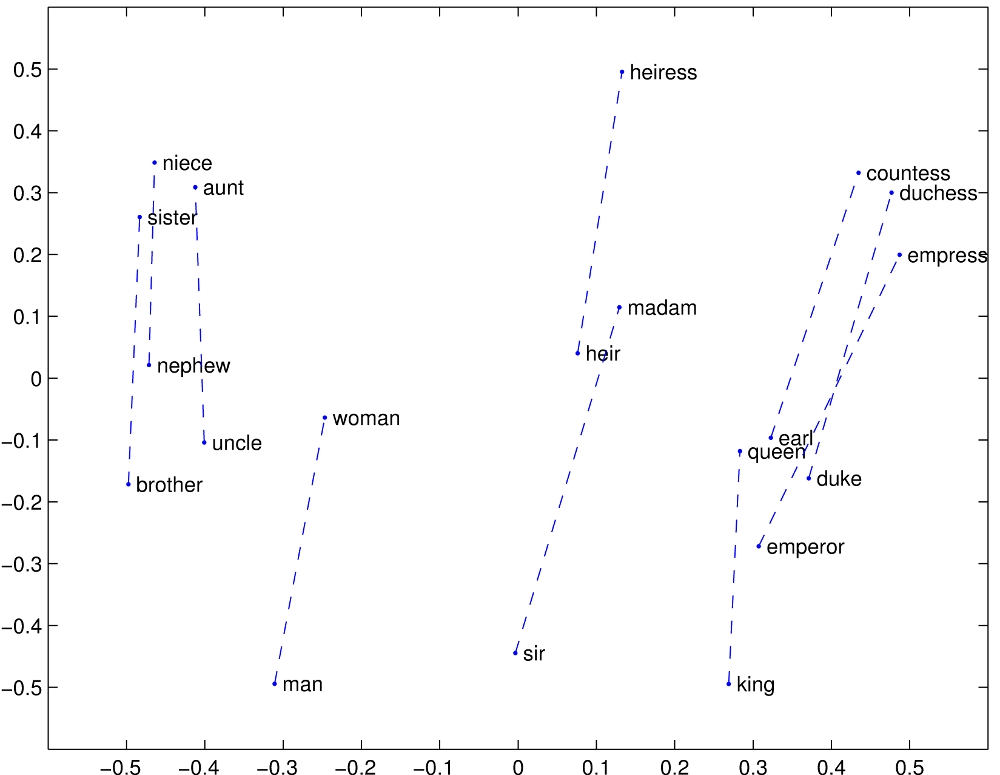
\includegraphics[width=0.6\textwidth]{img/man_woman.jpg}
  \end{center}
\end{frame}

\subsection{Attention Models}

\begin{frame}{Attention models}
  \begin{itemize}
  \item Developed for seq-to-seq task
  \item State of the art in machine translation
  \end{itemize}
  \begin{center}
    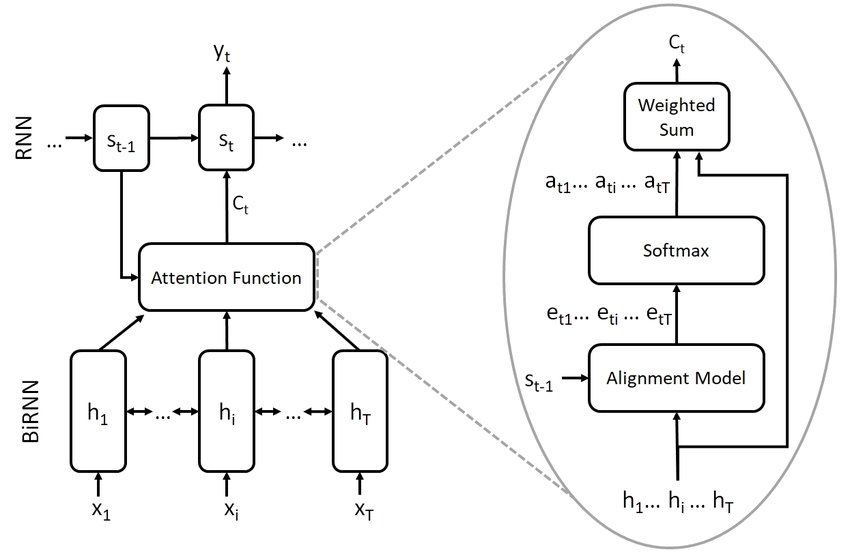
\includegraphics[width=0.6\textwidth]{img/attention.jpg}
  \end{center}  
\end{frame}

\subsection{Hierarchical models}
\begin{frame}{Hierarchical models}
  
\end{frame}

\subsection{\acs{bert}}
\begin{frame}{\acf{bert}}
  
\end{frame}

\section{Materials and Methods}

\subsection{Datasets}
\begin{frame}{Dataset}
  \begin{itemize}
  \item \alert{$1\,592\,385$} anatomopathological exam results
    \begin{itemize}
    \item From \alert{Tuscany} cancer registry
    \item In period \alert{2004-2013}
    \end{itemize}
  \item \alert{$94\,524$} ($6\%$) labeled
  \end{itemize}
  \begin{block}{Structure}
    \begin{itemize}
    \item 3 text \alert{fields}: macroscopy, diagnosis, anamnesis
    \item field \alert{length} from 0 to 1368 (quartiles 34, 62, 134)
    \end{itemize}
  \end{block}
\end{frame}

\begin{frame}{Preparation}
  \begin{itemize}
  \item Data comes in \alert{two} tables to merge:
    \begin{enumerate}
    \item neoplasm table, containing administrative and clinical variables
    \item histology table, containing the text fields
    \end{enumerate}
    \begin{itemize}
    \item there are neoplasms without histology associated
      \begin{itemize}
      \item (register have access to more data)
      \end{itemize}
    \item there are histologies without neoplasm associated
      \begin{itemize}
      \item (not tumor biopsies) 
      \end{itemize}
    \end{itemize}
  \item The 3 text fields are \alert{merged}
  \end{itemize}
\end{frame}

\subsection{Models}
\begin{frame}{Models}
  \begin{description}
  \item[\svm] \alert{\acs{svm}} trained on \alert{\acs{tfidf}} representations using \alert{unigrams}
  \item[\svmb] \alert{\acs{svm}} trained on \alert{\acs{tfidf}} using \alert{unigrams} and \alert{bigrams}
  \item[\lstmng] \alert{\acs{lstm}} trained on \alert{\acs{tfidf}} using
    \alert{bigrams}
  \item[\lstmc] mixed \alert{convolutional} and \alert{\ac{lstm}} trained on
    \alert{\acs{glove}}
  \item[\lstmb] \alert{\acs{lstm}} trained on \alert{\acs{glove}}
  \item[\gru] \alert{\acs{gru}} trained on \alert{\acs{glove}}
  \item[\maxp] \alert{\acs{gru}} with \alert{max} pooling trained on \alert{\acs{glove}}
  \item[\softmax] \alert{\acs{gru}} with \alert{attention} trained on \alert{\acs{glove}}
  \item[\maxi] \alert{\acs{gru}} with \alert{max} pooling, in \alert{interpretable} setting, trained on \alert{\acs{glove}}
  \item[\softmaxi] \alert{\acs{gru}} with \alert{attention}, in \alert{interpretable} setting, trained on \alert{\acs{glove}}
  \item[\maxh] \alert{hierarchical \acs{gru}} with \alert{max} pooling trained on \alert{\acs{glove}}
  \item[\softmaxh] \alert{hierarchical \acs{gru}} with \alert{attention} trained on \alert{\acs{glove}}
  \item[\bert] \alert{pretrained} on unlabeled data and \alert{fine tuned} with labeled data
  \end{description}
\end{frame}

\begin{frame}{\lstmng, \lstmc, \lstmb}
  \begin{figure}
  \centering
  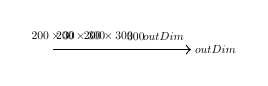
\begin{tikzpicture}[node distance = 0.1cm, auto]
    \begin{scope}[scale=0.7, transform shape]
    \begin{scope}[start chain, every node/.style={on chain}, node distance = \schemeNodeDistance]
      \nodeInput();
      \nodeEmbedding();
      \node[support] (emb) {};
      \nodeLstm();
      \node[support] (lstmA) {};
      \nodeLstm();
      \node[support] (lstmB) {};
      \nodeAvg();
      \node[support] (avg) {};
      \nodeRelu();
      \node[support] (relu) {};
      \nodeSoftmax();
      \node[dataLabel, joined] {$outDim$};
    \end{scope}
    \node[dataLabel, above=of emb] {$200\times 30$};
    \node[dataLabel, above=of lstmA] {$200\times 300$};
    \node[dataLabel, above=of lstmB] {$200\times 300$};
    \node[dataLabel, above=of avg] {$300$};
    \node[dataLabel, above=of relu] {$outDim$};
    \end{scope}
  \end{tikzpicture}
  \caption{Scheme for \lstmng{} model.}
\end{figure}

\begin{figure}
  \centering
  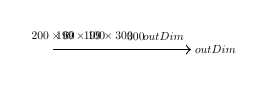
\begin{tikzpicture}[node distance = 0.1cm, auto]
    \begin{scope}[scale=0.7, transform shape]
      \begin{scope}[start chain, every node/.style={on chain}, node
      distance = \schemeNodeDistance]
      \nodeInput();
      \nodeGlove();
      \node[support] (glove) {};
      \nodeConv();
      \node[support] (conv) {};
      \nodeLstm();
      \node[support] (lstm) {};
      \nodeAvg();
      \node[support] (avg) {};
      \nodeRelu();
      \node[support] (relu) {};
      \nodeSoftmax();
      \node[dataLabel, joined] {$outDim$};
    \end{scope}
    \node[dataLabel, above=of glove] {$200\times 60$};
    \node[dataLabel, above=of conv] {$199\times 100$};
    \node[dataLabel, above=of lstm] {$199\times 300$};
    \node[dataLabel, above=of avg] {$300$};
    \node[dataLabel, above=of relu] {$outDim$};
  \end{scope}
  \end{tikzpicture}
  \caption{Scheme for \lstmc{} model.}
\end{figure}

\begin{figure}
  \centering
  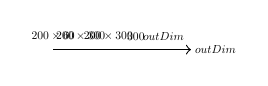
\begin{tikzpicture}[node distance = 0.1cm, auto]
    \begin{scope}[scale=0.7, transform shape]
    \begin{scope}[start chain, every node/.style={on chain}, node distance = \schemeNodeDistance]
      \nodeInput();
      \nodeGlove();
      \node[support] (glove) {};
      \nodeLstm();
      \node[support] (lstmA) {};
      \nodeLstm();
      \node[support] (lstmB) {};
      \nodeAvg();
      \node[support] (avg) {};
      \nodeRelu();
      \node[support] (relu) {};
      \nodeSoftmax();
      \node[dataLabel, joined] {$outDim$};
    \end{scope}
    \node[dataLabel, above=of glove] {$200\times 60$};
    \node[dataLabel, above=of lstmA] {$200\times 300$};
    \node[dataLabel, above=of lstmB] {$200\times 300$};
    \node[dataLabel, above=of avg] {$300$};
    \node[dataLabel, above=of relu] {$outDim$};
    \end{scope}
  \end{tikzpicture}
  \caption{Scheme for \lstmb{} model.}
\end{figure}
\end{frame}

\begin{frame}{\gru, \maxp, \softmax}
  \begin{block}{Plain model}
  \begin{align*}
  e_t &= E(x_t;\theta^e)\\
  h^f_t &= F(e_t,h^f_{t-1};\theta^f)\\
  h^r_t &= R(e_t,h^r_{t+1};\theta^r)\\
  u_t &= G(h_t;\theta^h)\\
  \phi &= A(\vect{u};\theta^a)\\
  f(\vect{x}) &= g(\phi;\theta^c)
  \end{align*}    
  \end{block}
  \begin{itemize}
  \item $\phi=(h^f_T,h^r_1)$ (in this case $G$ is the identity
    function)
  \item
    $\phi = \sum_t a_t(\vect{u};\theta^a) u_t$, $a_t(\vect{u};\theta^a) = \frac{e^{\langle c, c_t\rangle}}
    {\sum_i{e^{\langle c, c_i\rangle}}}$, $c_t=C(\vect{u};\theta^a)$
\item $\phi_j = \max_t u_{j,t}$
\end{itemize}
\end{frame}

\begin{frame}{\maxi, \softmaxi}
  \begin{block}{Interpretable model}
    \begin{align*}
  e_t &= E(x_t;\theta^e)\\
  h^f_t &= F(e_t,h^f_{t-1};\theta^f)\\
  h^r_t &= R(e_t,h^r_{t+1};\theta^r)\\
  u_t &= G(h_t;\theta^h)\\
  f(\vect{x}) &= A(\vect{u};\theta^a)
\end{align*}
  \end{block}
  \begin{itemize}
  \item
    $\phi = \sum_t a_t(\vect{u};\theta^a) u_t$, $a_t(\vect{u};\theta^a) = \frac{e^{\langle c, c_t\rangle}}
    {\sum_i{e^{\langle c, c_i\rangle}}}$, $c_t=C(\vect{u};\theta^a)$
\item $\phi_j = \max_t u_{j,t}$
\end{itemize}
\end{frame}

\begin{frame}{\maxh, \softmaxh}
  \begin{block}{Hierarchical model}
    \begin{align*}
  e_{s,t} &= E(x_{s,t};\theta^e)\\
  h^f_{s,t} &= F(e_{s,t},h^f_{s,t-1};\theta^{f})\\
  h^r_{s,t} &= R(e_{s,t},h^r_{s,t+1};\theta^{r})\\
  u_{s,t} &= G(h_{s,t};\theta^{h})\\
  \phi_s &= A(\vect{u}_s;\theta^{a})\\
  \bar{h}^{f}_{s} &= \bar{F}(\phi_{s},\bar{h}^{f}_{s-1};\bar{\theta}^{f})\\
  \bar{h}^{r}_{s} &= \bar{R}(\phi_{s},\bar{h}^{r}_{s+1};\bar{\theta}^{r})\\
  \bar{\phi} &= \bar{A}(\bar{\vect{h}};\bar{\theta}^{a})\\
  f(\vect{x}) &= g(\bar{\phi};\theta^c)
\end{align*}
  \end{block}
\end{frame}


\section{Experiments}

\subsection{Bag-of-words, word vectors, \acs{svm}, deep learning}

\subsection{Aggregation and interpretability}

\subsection{Aggregation, interpretability, hierarchical}

\section{Conclusions}





\begin{frame}
  \begin{center}
    \textbf{\calligra\Huge The End.}\\
    
\includegraphics[width=5cm]{img/ornament.eps}\\[1cm]
    {\huge\calligra Questions? Thank you!}
  \end{center}
\end{frame}


%\appendix
\backupbegin

\begin{frame}[allowframebreaks]{Bibliography}
  \scriptsize
  %\nocite{*}
  \bibliography{slides}
\end{frame}


\backupend

\end{document}

%%% Local Variables:
%%% mode: latex
%%% TeX-master: t
%%% End:
